%TO DO LIST
%CHECK EMAIL
%CHECK REVIEWS
%EVERTHING GREEN
%CHECK INDENT AFTER SECTION TITLES
\documentclass[a4paper,twoside]{article}

\usepackage[utf8]{inputenc} 
%\usepackage{mathptmx}
%\usepackage{textcomp}
 \usepackage{multirow}
\usepackage{epsfig}
\usepackage{subfigure}
\usepackage{calc}
\usepackage{amssymb}
\usepackage{amstext}
\usepackage{amsmath}
\usepackage{amsthm}
\usepackage{multicol}
\usepackage{pslatex}
\usepackage{apalike}
\usepackage{SCITEPRESS}     % Please add other packages that you may need BEFORE the SCITEPRESS.sty package.

\subfigtopskip=0pt
\subfigcapskip=0pt
\subfigbottomskip=0pt

\begin{document}

\title{A Semiautomatic Process Model Verification Plug-in based on Process Modeling Guidelines}
%FIXEMAIL
\author{\authorname{Valter Helmuth Goldberg Júnior\sup{1}, Lucineia Heloisa Thom\sup{1} José Palazzo Moreira de Oliveira and Diego Toralles Avila\sup{1}}
	\affiliation{\sup{1}Department of Informatics, Federal University of Rio Grande do Sul, UFRGS, Porto Alegre, Brazil}
	\email{\{EMAILDOWALTER,lucineia,palazzo,dtavila\}@inf.ufrgs.br}
}

\keywords{Business Process, BPMN, Ontology, Process Model Quality, Modeling Guidelines}


%CASE STUDY? What did Pimenta say?
\abstract{Designing process models easy to understand is a complex task.  Process analysts must rely on the experience of expert systems managers to achieve process models with high comprehensibility, also known as pragmatic quality. In the literature, this integration procedure is portrayed as process modeling guidelines that help modelers avoid common issues that hinder the comprehension of the process model. In this paper, we show a method for semi-automatically verifying business process models according to process modeling guidelines. This method uses the BPMN Ontology and the ontology editor \textit{Protégé} to assist the modeler with validation of the process model's syntax before following with verifying its pragmatic quality. The validation of the method was applied to a collection of 31 process models andthe results are show in the case study here described.}

\onecolumn \maketitle \normalsize \vfill

\section{INTRODUCTION} \label{Introduction}

%What is BPM
%DONE?
\noindent Business Process Management (BPM) is a discipline that provides a systematic approach to manage an organization's work by modeling, analyzing, improving and controlling its business processes (hereafter called processes, for simplification). It contributes to the increase of productivity and reduction of costs through more effective, more efficient and more adaptable processes \cite{aalst:2013}. %As such, we are increasingly worried about the quality of our processes, as we base the value of a business on top of the models generated by the modeling of our processes in BPM.

Through the use of BPM, organizations continually seek to improve the quality of their processes. However, studies analyzing industry process model collections reveal that many process models contain issues that harm its quality, such as control flow errors, badly designed structures and layouts or incorrect labeling \cite{Mendling2008a} \cite{Leopold2016}. With the process modeling being a key part of BPM, it is important that we try to prevent these issues if we expect processes of better quality.

%Model and Modeling - To work with process we need a model of said process. Modeling is a fundamental task in BPM.
%Problem - Modeling is hard and not objective. Some models are better than others
%I have to point out that many models are badly created, that this is an actual problem in reality, not that "Modeling is hard". Instead, let this paragraph tell WHY modeling is hard.
%ALSO, "Modeling" or "Modelling". This paper will be presented on the EU (I think), which spelling is commonly used there?

It is widely accepted that modeling a process is a difficult task \cite{Mendling2010}. This is usually due to the complexity of the modeling notation, its many different elements and their respective semantics \cite{Leopold2016}. Choosing the appropriate representation depends upon the expertise or the guidance of an experienced modeler, that may greatly influence the quality of the resultant process model. We need to consider that the use of process modeling tools can help in this regard, they cannot guarantee a process model's correctness nor its comprehensibility.


%Guidelines - There are "rules of thumb" to modeling. We want to verify said rules with some formality.
%guidelines "solve" the quality challenge, they do reduce complexity and prevent errors, they are many, etc, BUT their use is not that widespread, especially in professional tools.

One way to solve this challenge and help the beginner modelers is to consolidate the knowledge of experienced modelers in process modeling guidelines, whose purpose is to help the user reduce the complexity and the number of errors in a process model through the restriction of undesirable constructs. Many guidelines have been proposed by both practitioners \cite{Silver2009} \cite{White2008} \cite{Allweyer2010} and researchers \cite{Becker2000} \cite{Mendling2007} \cite{Vanderfeesten2008} \cite{Correia2012}. Once it is verified that a process model is following a set of guidelines, we can presume that it has good comprehensibility.

%Syntax before comprehensibility
However, using guidelines to verify a process model doesn't make sense if it isn't syntactically correct. Any knowledge extracted from an incorrect process model has its validity compromised because, while you may be able to understand it, you may doubt whether it is what the modeler intended to represent \cite{Reijers2015}. Therefore, one must check if a process model is correct before considering it's comprehensibility.


%Ontology - Verifies correctness
It is possible to verify the correctness of process models in  different ways. One of these is by the means of ontologies. Ontology is the study of being, which pursues to represent the world as entities, categories and relations \cite{Mendling2008}. In a more practical setting, an ontology provides an approach to define types, properties and relations. Given this, we can use an ontology for process models as a meta-model to verify a process model's correctness.


%Hypothesis and %Objectives
Following these lines, the purpose of this paper is to show how the use of ontologies should assist in the identification of problems that reduce a process model's comprehensibility. To do that, it is necessary to submit a process model to a process model ontology processor and, after that, verify it using a set of process modeling guidelines, pointing out any problems that can be improved upon.


%PaperStructure
This paper is organized as follows: Section \ref{RelatedWorks} outlines previous works related to the verification of process models. Section \ref{Background} shortly introduces the basic concepts used in this paper. Section \ref{Methodology} displays the context we choose to work with and the method we developed. Section \ref{CaseStudy} presents our case study and our results. Section \ref{Conclusion} closes the paper with our conclusions.

\section{RELATED WORKS}\label{RelatedWorks}

%Verification Works

%Through Correctness
\noindent The verification of business process models is nothing new, in fact, numerous researches addressed this subject. The difference is that most of these researches are concerned with issues of correctness of a process model. In \cite{Mendling2008}, for example, the author proposes two different approaches to verifying soundness of a process model draw using Event-Process-Chains.
	
%Through Metrics 
Evaluating and reducing the complexity of a process model is harder to achieve. It is not possible to measure a process complexity directly and, as a consequence, many metrics have been proposed that try to solve this problem indirectly \cite{Vanderfeesten2007} \cite{Mendling2008b} \cite{Gruhn2006}. The validity of these metrics is evidenced through statistical experiments, where process models are judged both by the metrics and by people with varying levels of modeling experience \cite{Cardoso2006a} \cite{Sanchez-Gonzalez2008}.

%Through Guidelines
%REWRITE
As it was mentioned, many authors proposed guidelines for modeling processes, with repeated guidelines that had already been proposed, with only few small variations in the details. In \cite{Moreno-MontesdeOca2014}, these repeats were gathered from a systematic review about business process modeling quality from over a 100 proposed in the literature and turned into 27 unified guidelines.  

Some of the existing BPMN tools try to provide some support for creating good process models. Based on the guidelines found in the refered article, a study \cite{MoniqueSnoeckIsel2015} was performed to test how extensive was, at the time, the support of the popular BPMN tools in creating good process models. From this, we can learn that the Signavio \footnote{www.signavio.com} modeler tool provides the best amount of support for modeling processes using guidelines. 


\section{BASIC NOTIONS}\label{Fundamentals}\label{Background}

%Modeling %BPMN %Problems
%IMPROVE? Should I insert BPMN element types?
\noindent The modeling task of BPM is often done using the Business Process Model and Notation (BPMN). BPMN was developed by the Object Management Group (OMG), with the purpose of consolidating the many existing notations for process models in a single standard. This standard should provide an easy to understand notation to all stakeholders \cite{OMGObjectManagementGroup2015}. However, BPMN does not teach modelers how to use it's elements in the creation of simple and expressive process models. The consequence of this is that it's hard to achieve a good level of quality in BPMN process models.


%Qualities
%REFERENCES
This difficulty motivated the creation of many frameworks that try to define what is the quality of a process model and classify the different quality types that compose it. Examples of these efforts are the SEQUAL Framework \cite{krogstie2012}, the Guidelines of Modeling (GoM) \cite{Schuette1998} and, more recently, the SIQ framework \cite{Reijers2015}), in which we base the present work. The SIQ framework defines process model quality as made of three basic quality types:

%REFERENCE OF SOUND
\begin{itemize}
	\item \textbf{Syntactic Quality} identifies if a process model conforms to the rules defined by the notation utilized to create it. In other words, if a process model follows the syntax and the vocabulary of its modeling language, then it is possible to verify that process model and declare it to be correct. To do so, the verification must check the static proprieties of a process model - how different types of elements are used and combined - and its behavioral proprieties - the process modeled should not reach a deadlock and must be completed properly, i.e the process model is \textit{sound}.
	\item \textbf{Semantic Quality} bears the connection between a process model and the real world process it's supposed to represent. Checking a process model's semantic quality is, basically, making sure it is valid - all elements of the process model correctly represent the real world - and complete - there are no real world process parts that are missing in the process model. This check is simply called validation and, if it passes, the process model is ascertained to be true.
	\item \textbf{Pragmatic Quality} characterizes the comprehensibility of a process model. It is the certification that a user's interpretation of a process model is equal to the real world process. If done, the process model is said to be understood.
\end{itemize}

%Syntactic is basis for the others

\begin{figure}
	\centering
	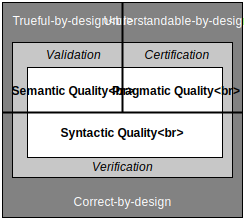
\includegraphics[scale=0.8]{SIQFramework.png}
	\caption{The SIQ Framework (adapted from \cite{Reijers2015})}
	\label{SIQFigure}
\end{figure}

Syntactic quality is the basis for the other two qualities. As mentioned before, it is not reasonable to consider the comprehensibility of a process model if it is not syntactically correct. The same can be expreseed on its semantic quality. The verification of a process model must be done before its validation or certification.

%TODO - Mention OWL?
%BPMN Ontology
As previously explained, it's possible to do this verification using an ontology. More specifically, we can use an ontology design to serve as a meta-model for a process modeling notation. In the case of BPMN, there exists what is called the \textit{BPMN Ontology} \cite{Rospocher2014foisbpmn}, which supports the mapping of a BPMN process model into elements of the ontology, while preserving the relations and strutures between the process model elements. That way, we can use an inference engine to verify the mapped process model, to check if the static properties of BPMN model, i.e its structure, is correct according to the BPMN syntax.


%To verify these guidelines, we need to transform the model from the BPMN standard into a more formal one, which in this case is an ontology, because, in computer science, the most common definition of an ontology is an explicit and formal specification of a shared conceptualization \cite{borst1997ontology, Gruber1995907, Studer1998161}. The transformation between BPMN and an ontology is done through the use of the already existing \textit{BPMN Ontology} \cite{Rospocher2014foisbpmn}. This allows us to verify the process model, or more precisely its structure, through the use of an ontological reasoner. 
%The Table \ref{BPMNOntologyMapping} shows how the mapping is done.

%Guidelines
%7PMG
Finally, assuming the process model is indeed correct, we can try to ensure its pragmatic quality, which, in this case, is done by checking via the use of process modeling guidelines.  In \cite{Mendling2010}, seven process modeling guidelines (7PMG) have been proposed that are "thought to be helpful in guiding users towards improving the quality of their models, in the sense that these are likely (1) to become comprehensible to various stakeholders and (2) to contain few syntactical errors". These guidelines have been built upon empirical insights and, as such, provide a short but meaningful set of rules. They are as follows:
\begin{enumerate}
	\item[G1] Use as few elements in the model as possible.
	\item[G2] Minimize the routing paths per element.
	\item[G3] Use one start and one end event.
	\item[G4] Model as structured as possible. 
	\item[G5] Avoid OR routing elements.
	\item[G6] Use verb-object activity labels.
	\item[G7] Decompose a model with more than 50 elements.
\end{enumerate}

%SWTICH NAME
\section{A METHOD FOR VERIFYING PROCESS MODELS BASED ON PROCESS MODELING GUIDELINES}\label{Methodology}
\begin{table}[]
	\centering
	\caption{Parameters tested for each guideline from 7PMG}
	\label{Metrics}
	\begin{tabular}{|c|c|}
		\hline
		7PMG & Metrics and Comparisons \\ \hline
		G1 & Number of Elements $>$ 30 \\ \hline
		G2 & Highest Element Degree $>$ 7 \\ \hline
		G3 & \begin{tabular}[c]{@{}c@{}}Number of StartEvents $>$ 1\\ Number of End Events $>$ 1\end{tabular} \\ \hline
		G4 & Number of Splits $\neq$ Number of Joins \\ \hline
		G5 & Number of OR Gateways $>$ 0 \\ \hline
		G6 & Wordnet \\ \hline
		G7 & Number of Elements $>$ 30 \\ \hline
	\end{tabular}
\end{table}

\begin{table*}[]
	\caption{BPMN $\Rightarrow$ Ontology Mapping}
	\label{bpmnOntologyMapping}
	\centering
	\begin{tabular}{| c |c |c |}
		\hline
		BPMN & Ontology & Example \\
		\hline
		Element Type & OWL Class & Activity, Gateway \\\hline
		Element Instance & Individual Named & Task 1: Submit Report \\  \hline
		Attribute & Object Property & Label="Name" \\\hline
		Attribute Value & Data Property & Name:String="Task 1: Submit Report" \\ 
		\hline
	\end{tabular} 
\end{table*}

\noindent To fulfill the purpose of this paper, we must specify a series of steps that, with the assistance of an ontology, allows us check a process model's pragmatic quality by verifying whether it follows the seven process modeling guidelines. However, before we can do this, there are some things that must be defined. 

To start with, we must decide how are the process models going to be represented. A few different notations for process models exist and each notation has different ways of how the process model is coded within a file. As may be implied from the previous section, the notation used in this work is BPMN 2.0. Models using this notation may be exported to the interchangeable format defined by OMG, which is a XML file with a specific schema and a .bpmn extension \cite{OMGObjectManagementGroup2015}. From this file, we can easily map elements from the process model into the an ontology, via the \textit{BPMN Ontology}.

Secondly, it is necessary to establish how to check whether or not a guideline is being followed by a process model. They must be expressed in such a way that they turn into a binary, yes or no question. To do that, each guideline must be associated to a process model indicator that can be measured and compared against expected optimal values. Based upon previous works \cite{Mendling2008} \cite{Recker2011} \cite{Mendling:2012}, the table \ref{Metrics} presents the indicators and the optimal values considered to check if the process model violates each guideline. Based on these, two guidelines show problems: G1 and G6.

%G1, the guideline for encouraging the use of less elements when modeling, becomes redundant with G7, which determines when a model should be decomposed. This happens because G1 is much more suited to be used when a model is being developed, when one can refrain from introducing a few elements instead of when the modeling is finished and the choice becomes of how the model can be decomposed. As a result, the metric measured for both guidelines is the same, requiring us to choose the more appropriate one for testing. In this case, since we are working with a model and not with modeling, the guideline G7 is more appropriate.


%REWRITE LAST?
G1, the guideline for encouraging the use of less elements when modeling, becomes redundant with G7, which determines when a process model should be decomposed. This happens because the indicator used for G1 is the same as the one used for G7. As a consequence, we need to choose which guideline is more appropriate for the proposed method. Since G1 is more suited to be used when a process model is being developed and the modeler can refrain from introducing a few elements, instead of when the modeling is finished, the guideline G7 is more appropriate.

G6, which tells us to label activities in the verb-object style, presents a problem in the complexity of checking the language of each label. This exceeds the scope of this work, since it requires the use of Natural Language Processing to identify the words of each label and compare them and their use against a thesaurus to define the label's context \cite{Gassen2014}. Therefore, we are ignoring this guideline.



Finally, it must be determined how an ontology will be loaded and edited. We chose to use the ontology editor \textit{Protégé} \footnote{http://protege.stanford.edu/}. \textit{Protégé} not only can verify the integrity of ontologies using an inference engine, it is also easily extensible through the use of plugins. The majority of our method was built using this extensibility. %Both features will be helpful in our method. 

\noindent Having made these decisions, we specified a method to verify process models based on the seven process modeling guidelines. To do so, this method verifies a process model syntax using an ontology and its inference engine and then check the process model using the guidelines.

The first step of the method is to prepare \textit{Protégé} for instantiating BPMN models. The BPMN ontology is loaded to support the mapping of elements from BPMN to the ontology by serving as the meta-model containing the structuring rules of BPMN.

Following this, the individual elements from the BPMN models can be extracted and instantiated into the ontology by a Java plugin which reads the .bpmn file of the process models and extracts its tasks, gateways, sequence flows and messages. After that, this same plugin uses the OWL-API to create individuals for each element, mapping and instantiating them according to each type described by the BPMN Ontology. The table \ref{bpmnOntologyMapping} shows the mapping.

\begin{figure*}
	\includegraphics[width=\textwidth ]{method.png}
	\caption{Steps to verify process models based on process modeling guidelines}
	\label{methodFigure}
\end{figure*}

\begin{table}[]
	\centering
	\caption{Recommended Actions for each tested guideline}
	\label{RecommendedActions}
	\begin{tabular}{|c|p{5.5cm}|}
		\hline
		7PMG & Recommended Action \\ \hline
		G2 & Reduce the number of sequence flows connected to a single element \\ \hline
		G3 & Restructure the process model to reduce the number of Start and End events \\ \hline
		G4 & Restructure the process model to have the same number of Split and Joins \\ \hline
		G5 & Restructure the process model to remove the OR Gateways \\ \hline
		G7 & Decompose the process model \\ \hline
	\end{tabular}
\end{table}

Once the entire process model has been instantiated in the ontology, the \textit{Protégé}  verifies if the process model is syntactically correct.  Using \textit{Protégé} inference engine, we can verify the ontology's integrity and, if this is successful, it can be assumed that the structure of the BPMN model is syntactically correct, since any syntactical error in the process model's structure would violate the ontology's integrity according to the BPMN Ontology.

The final steps of this method are checking the process model according the seven process modeling guidelines and recommending alterations based upon the results. Another Java Plugin checks the process model's indicators and, for each violated guideline, recommends actions according to the table \ref{RecommendedActions}.

The entire series of steps is as follow (figure \ref{methodFigure}):

\begin{enumerate}
	\item Load the BPMN Ontology in \textit{Protégé}
	\item Extract each individual element from a BPMN model.
	\item Instantiate each extracted element in \textit{Protégé} via OWL-API and using the BPMN Ontology.
	\item Use \textit{Protégé}'s inference engine to verify the integrity of the new ontology.
	\item Check if the process model's indicators obey the limits defined by the modeling guidelines.
	\item Recommend alterations to the process model for each guideline not followed.
\end{enumerate}

%To verify the process model according to the 7PMG, a plug-in for Protégé was developed, in which each guideline proposed had to be represented. For most guidelines (G1, G2, G3, G5, G7), we can do this using a simple test performed on top of a process model's metrics. For G4, we simplify the guideline by measuring the number of splits and joins for each type of gateway. If that number is different then G4 has been disobeyed. Finally, G6 involves natural language processing for analyzing the syntax of each label, which is something outside of the scope of the work presented in this paper, therefore it has been left out. Table \ref{Metrics} shows each rule and associated metric being tested. Finally, the results of the verification are shown using a another plug-in in Protégé. The result of the test of each guideline is show with a "True" or "False" value.


\begin{table*}[]
	\centering
	\caption{Statistics for the indicators related to the guidelines G2, G3, G5, G7}
	\label{MetricsExtracted}
	\begin{tabular}{|c|c|c|c|c|c|}
		\hline
		& \begin{tabular}[c]{@{}c@{}}Highest \\ Connectivity Degree\end{tabular} & Nº Start Events & Nº End Events & Nº OR Gateways & Nº Elements \\ \hline
		Average & & 2.20513 & 2.25641 &  0.28125 & 24.79487 \\ \hline
		Std. Deviation & & 2.00236 & 1.96974 &  0.85135 & 17.71288 \\ \hline
		Minimum & & 1 & 1 &  0 & 6 \\ \hline
		Maximun & & 13 & 13 &  4 & 98 \\ \hline
		Median & & 2 & 2 &  0 & 21 \\ \hline
	\end{tabular}
\end{table*}

\section{CASE STUDY AND RESULTS}\label{CaseStudy}

\noindent To validate our method, we applied it to a collection of 31 BPMN models. These are models of the processes of a university, created by BPM students, verified and corrected by their professor and semantically validated by each process stakeholders. 

For each guideline used in the method, the associated indicators were extracted for a statistical analysis (as seen in tables \ref{MetricsExtracted} and \ref{MetricsGateways}). Based on these statistics, we have tried to predict whether most of the process models of this collection follow or not the process modeling guidelines. 



\begin{table}[]
	\centering
	\caption{Statistics for the indicators related to the guideline G4}
	\label{MetricsGateways}
	\begin{tabular}{|c|c|c|c|}
		\hline
		\multirow{2}{*}{}  & \multicolumn{3}{c|}{Splits - Joins Difference} \\ \cline{2-4} 
		& AND            & XOR           & OR            \\ \hline
		Average            & 0.125          & 0.53125       & -0.09375      \\ \hline
		Std. Deviation & 0.33601   & 1.39085   & 0.39016   \\ \hline
		Minimum            & 0              & -2            & -2            \\ \hline
		Maximun            & 1              & 4             & 0             \\ \hline
		Median             & 0              & 0.5           & 0             \\ \hline
	\end{tabular}
\end{table}

%TODO G2
For example, in the statistics for highest connectivity degree, associated with guideline G2, we see an average of NUM. If we sum this average with the standard deviation, it is possible to perceive that it's unlikely, assuming a normal distribution, that a random process model picked from our collection will have more than the recommended threshold for this guideline, which is five. Consequently, we can anticipate that the high majority of process models from the collection will follow the guideline. G5 is similar, since the average number of OR gateways is low, but not zero, and the standard deviation is almost 1, implying that a few process models do use OR gateways, up to the maximum of 4. For this reason, we suppose that a few process models violate this guideline, and our method shows this clearly.

For G3, on the other hand, we see the opposite situation, as the number of both start and end events has the high average (more than 2), compared to the recommended use of 1 event of each. This implies that most process models from the collection have multiple start and end event and, therefore, they do not follow G3. 

Analysis for guideline G4 is more complicated, since we define whether or not the process model is structured as the measure of the difference between the two indicators of the number of splits and the number of joins. Not only that, it is necessary to measure this difference for each different type of gateway. This balance means that the closer to zero is the average difference and the lower the standard deviation is then the more likely it is that the process models are structured.  We can clearly realize the opposite, however, since there is an imbalance of the number of XOR splits versus the number of XOR joins according to the that indicator. Also, the high standard deviation shows for each gateway indicates that most process models in the collection are not structured. Therefore, we predict that most process models of this collection infringe the guideline G4.

Finally, the statistics for G7 are slightly vague. The high, but not unreasonable, average for the measure of the number of elements suggest that the guideline is followed. Yet, the high standard deviation shows a hint that at least some process models do have more than 30 elements.

With all this information in mind, our expectations are that most process models violate guidelines G3 and G4, while following guidelines G2 and G5. Lastly, guideline G7 will a have a few violations.

\begin{table}[]
	\centering
	\caption{Number of violations Per guideline}
	\label{ViolationsPerGuideline}
	\begin{tabular}{|c|c|c|}
		\hline
		& Total Violations & Percent of Total \\ \hline
		G2 & 2 & 6.45\% \\ \hline
		G3 & 1 & 3.23\% \\ \hline
		G4 & 10 & 32.26\% \\ \hline %TOREDO. I know it's 21-22
		G5 & 4 & 12.90\% \\ \hline
		G7 & 8 & 25.81\% \\ \hline
	\end{tabular}
\end{table}

%REWRITE?
Comparing these conclusions with the results of the applied method (as show in table \ref{ViolationsPerGuideline}) shows that the predictions for guidelines G2, G4, G5 and G7 match the results. The results for guideline G3, however, is completely unexpected. 

Upon further analysis, we found a reason for this. Many process models of the collection have multiple pools or sub processes, which, according to the notation, require new start and end events, causing a distortion in the number of events that a process model has. Therefore, we must take said distortion into account for our statistical analysis. Nevertheless, our plugin that verifies process models is doing this correctly.





\section{CONCLUSIONS}\label{Conclusion}

\noindent Process models that follow the guidelines of process modeling are more likely to be understood by the process stakeholders. With the help of process modeling tools that support those guidelines, modelers can more easily represent and communicate the mechanisms of a process through the models, achieving higher levels of modeling quality that improve the work of an organization.

%CASE STUDY?
Through our case study, we have perceived the difficulty that beginner modelers experience in creating process models that follow modeling guidelines. The majority of process models in the collection have at least one aspect that is inefficient for the comprehension of it (table \ref{ModelsPerQuantityOfViolation}). It is observable that beginners need help in finding these inefficiencies and that this may only be accomplished if more support is given from the software modeling tools.

\begin{table}[]
	\centering
	\caption{Number of process models per quantity of violations}
	\label{ModelsPerQuantityOfViolation}
	\begin{tabular}{|c|c|}
		\hline
		& Number of Models \\ \hline
		No violations & 12 \\ \hline
		One violation & 14 \\ \hline
		Two violations & 4 \\ \hline
		Three violations & 1 \\ \hline
	\end{tabular}
\end{table}

In this paper it was shown that it is possible to semi-automatically verify process modeling guidelines with the assistance of the BPMN ontology. This procedure quickly analyzes the process models and recommend solutions to increase the pragmatic quality of the process model. %AMBIGUOUS

%Note that the BPMN ontology is not worried with modeling the process dynamic behavior
One limitation that must be acknowledged is related with the use of the BPMN ontology to check the syntax of the process model. While it is possible to verify the static proprieties of a process model, the BPMN ontology is not suited to specify  a process model's dynamic behavior \cite{Rospocher2014foisbpmn}. Therefore, we were not able verify a process model's entire syntactic quality.

While the method is by no means complete, as there are more guidelines in the literature beyond those applied here, we hope that this work brings attention to the necessity of accurate tool support for creating process models with high comprehensibility. We also believe that our work will provide a basis for future works in this area.

.

%\bibliographystyle{splncs03}
\bibliographystyle{apalike}
\bibliography{ArtigoVerificacao}
\end{document}